\section{Introduction}

%\haodong{Remember to shorten the main text to no more than 9 pages as soon as possible!! important}
Scaling laws~\citep{hestness2017deep,kaplan2020scaling,hoffmann2022training} have emerged as a central framework for characterizing the behavior of large language model (LLM) pre-training.
The Chinchilla scaling law~\citep{hoffmann2022training} established robust empirical trends in performance as a joint function of model size and dataset size under the one-pass training paradigm, in which each data point is used at most once.
This assumption, however, is becoming increasingly untenable.
The quest for more capable models has driven an unprecedented escalation in data requirements: from fewer than 10 billion tokens for GPT-2, to 300 billion for GPT-3~\citep{brown2020language}, 2 trillion for Chinchilla and LLaMA 2~\citep{hoffmann2022training, touvron2023llama}, and 36 trillion for Qwen3~\citep{yang2025qwen3}.
Projections further suggest that the pool of publicly available data may be exhausted as early as 2028~\citep{villalobos2024run}.

A common response to this emerging data scarcity is to train models for multiple epochs over the same dataset.
Recent empirical studies have begun to examine the consequences of such repetition: for example, \citet{muennighoff2023scaling} and \citet{xue2023repeat} show that moderate reuse can still yield competitive pre-training performance.
Yet the fundamental scaling behavior of multi-epoch training remains poorly understood—particularly from a theoretical standpoint.

In this paper, we study a fundamental question in understanding how multi-epoch training affects the data scaling laws: \textit{To what extent can training for $K$ epochs on $N$ samples be effectively seen as one-pass training with an increased number of data samples?}
% \kaifengclaw{Typo/grammar: 'does ... can be' is ungrammatical. Suggest: 'To what extent can training for $K$ epochs on $N$ samples be effectively viewed as one-pass training with a larger dataset?'}
Formally, let $\mathcal{L}(K, N)$ denote the expected loss of $K$-epoch training on $N$ samples. We define the \textit{effective dataset size} $N'(K, N)$ as the minimal number of samples in one-pass training that achieves a comparable or lower loss $\mathcal{L}(1, N') \leq \mathcal{L}(K, N)$.
In this paper, we are concerned with the ratio $E(K, N) = N'(K, N)/N$, which we term as the \textit{effective reuse rate} of the data, a key quantity that characterizes how many times larger the dataset must grow to match the same performance as $K$-epoch training (see the detailed version in \Cref{def:E_K}).
% \kaifengclaw{Typo/wording: 'we concern about' -> 'we are concerned with' or 'we focus on'; 'term as' -> 'term'.}


\begin{figure}[t]
    \vspace{-0.5in}
    \centering
    \begin{subfigure}[t]{0.32\linewidth}
         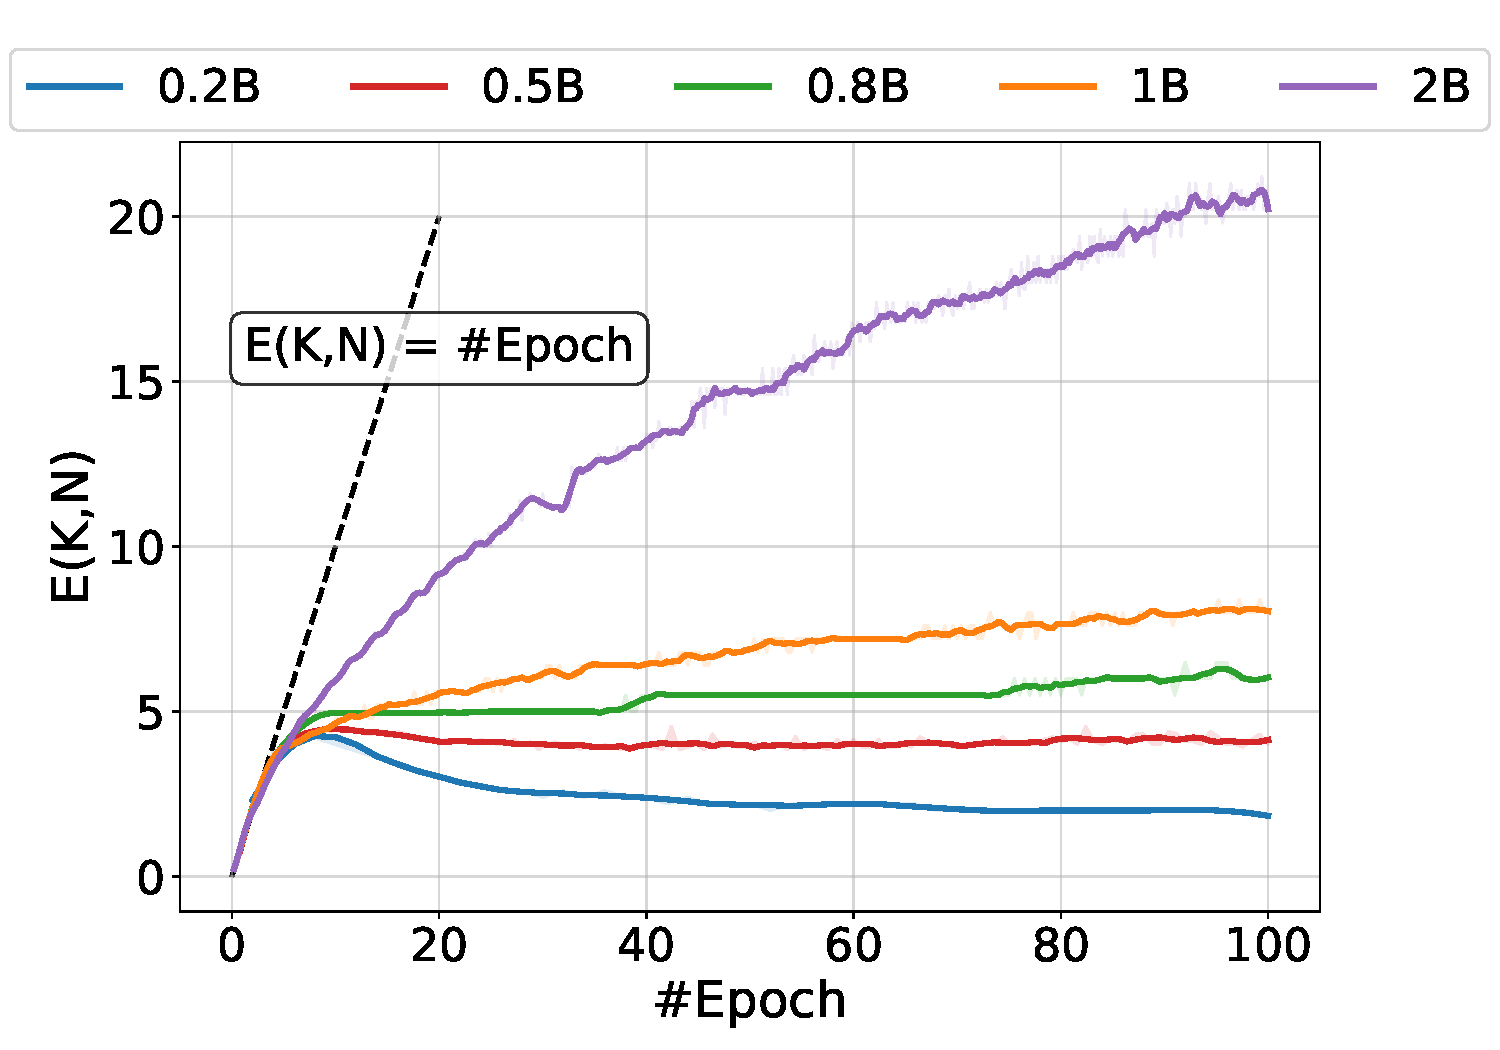
\includegraphics[width=\linewidth]{figs/E_k_smoothed_shaded.pdf}
        %\caption{The effective reuse rate $E(K,N)$ as a function of the epoch number $K$.}
        \caption{$E(K,N)$ as a function of $K$.}
        % \caption{The effective reuse rate $E(K,N)$ as a function of the number of training epochs $K$ for varying fresh data sizes $N$. The shaded regions represent the variability from the smoothed trend in different epochs.}
        \label{fig:ek-k}
    \end{subfigure}  
    \hfill
    \begin{subfigure}[t]{0.32\linewidth}
        % 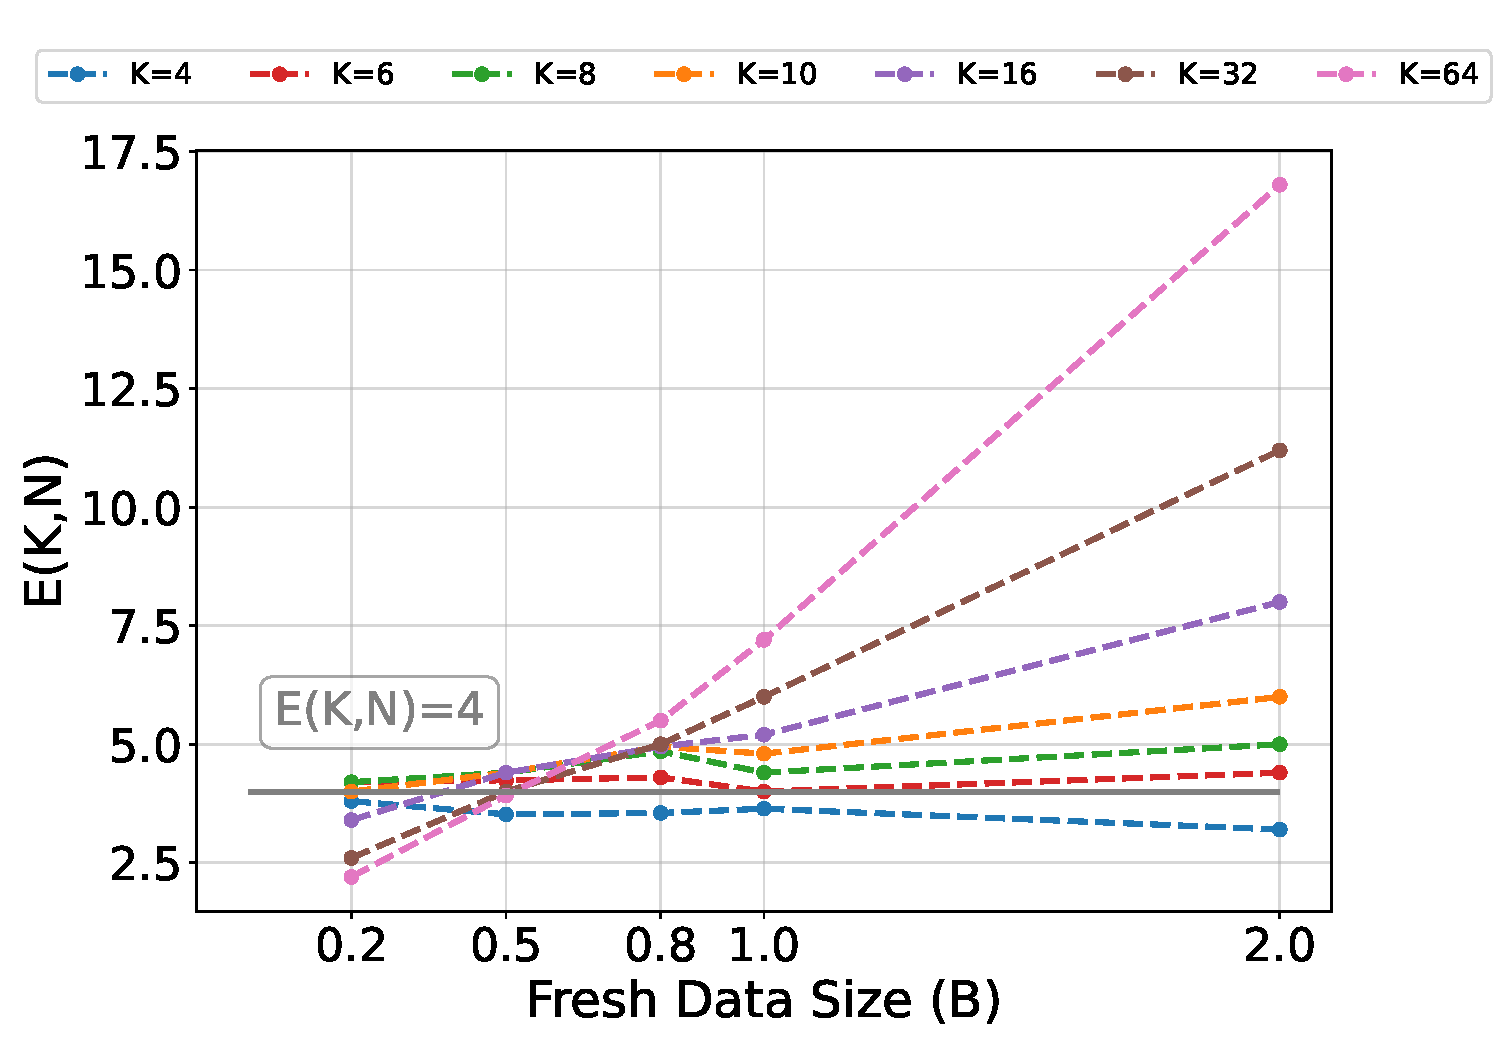
\includegraphics[width=\linewidth]{figs/E_k_over_fresh_data_size.pdf}
        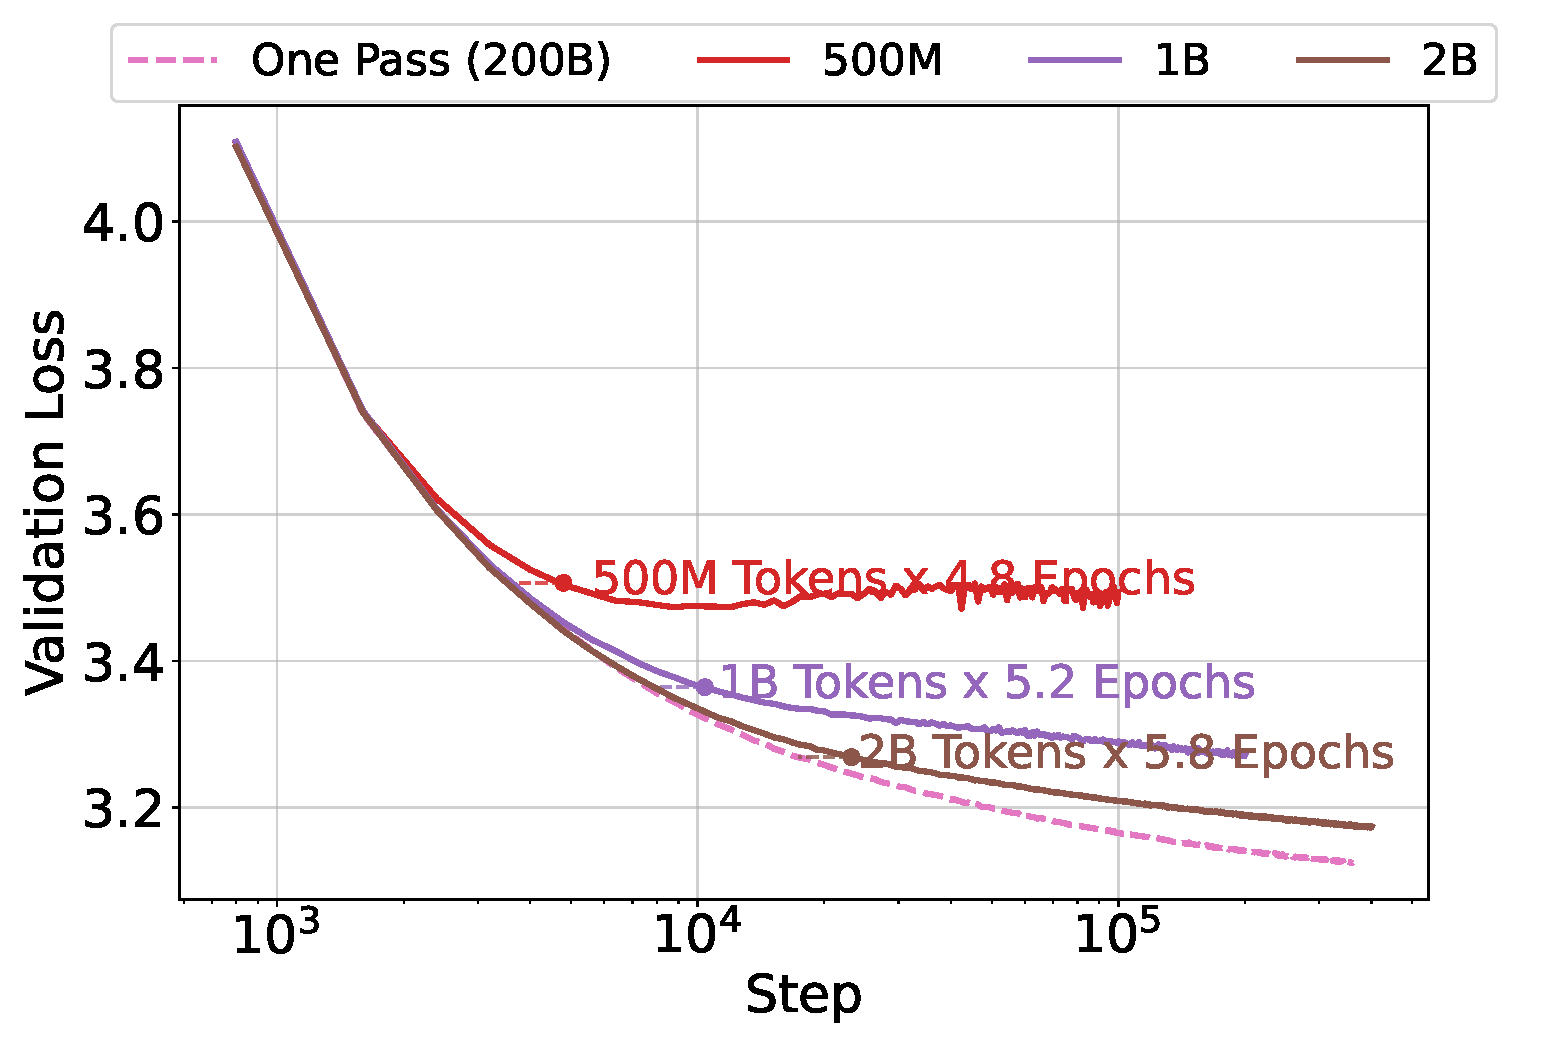
\includegraphics[width=\linewidth]{figs/loss_over_step_improved_ws3_ratio0.75_alpha0.9_exp.pdf}
        %\caption{Training loss as a function of training steps for different fresh data sizes.}
        \caption{Validation loss of one-pass and multi-epoch training runs.}
        \label{fig:loss-step}
    \end{subfigure}
    \hfill
    \begin{subfigure}[t]{0.33\linewidth}
        % 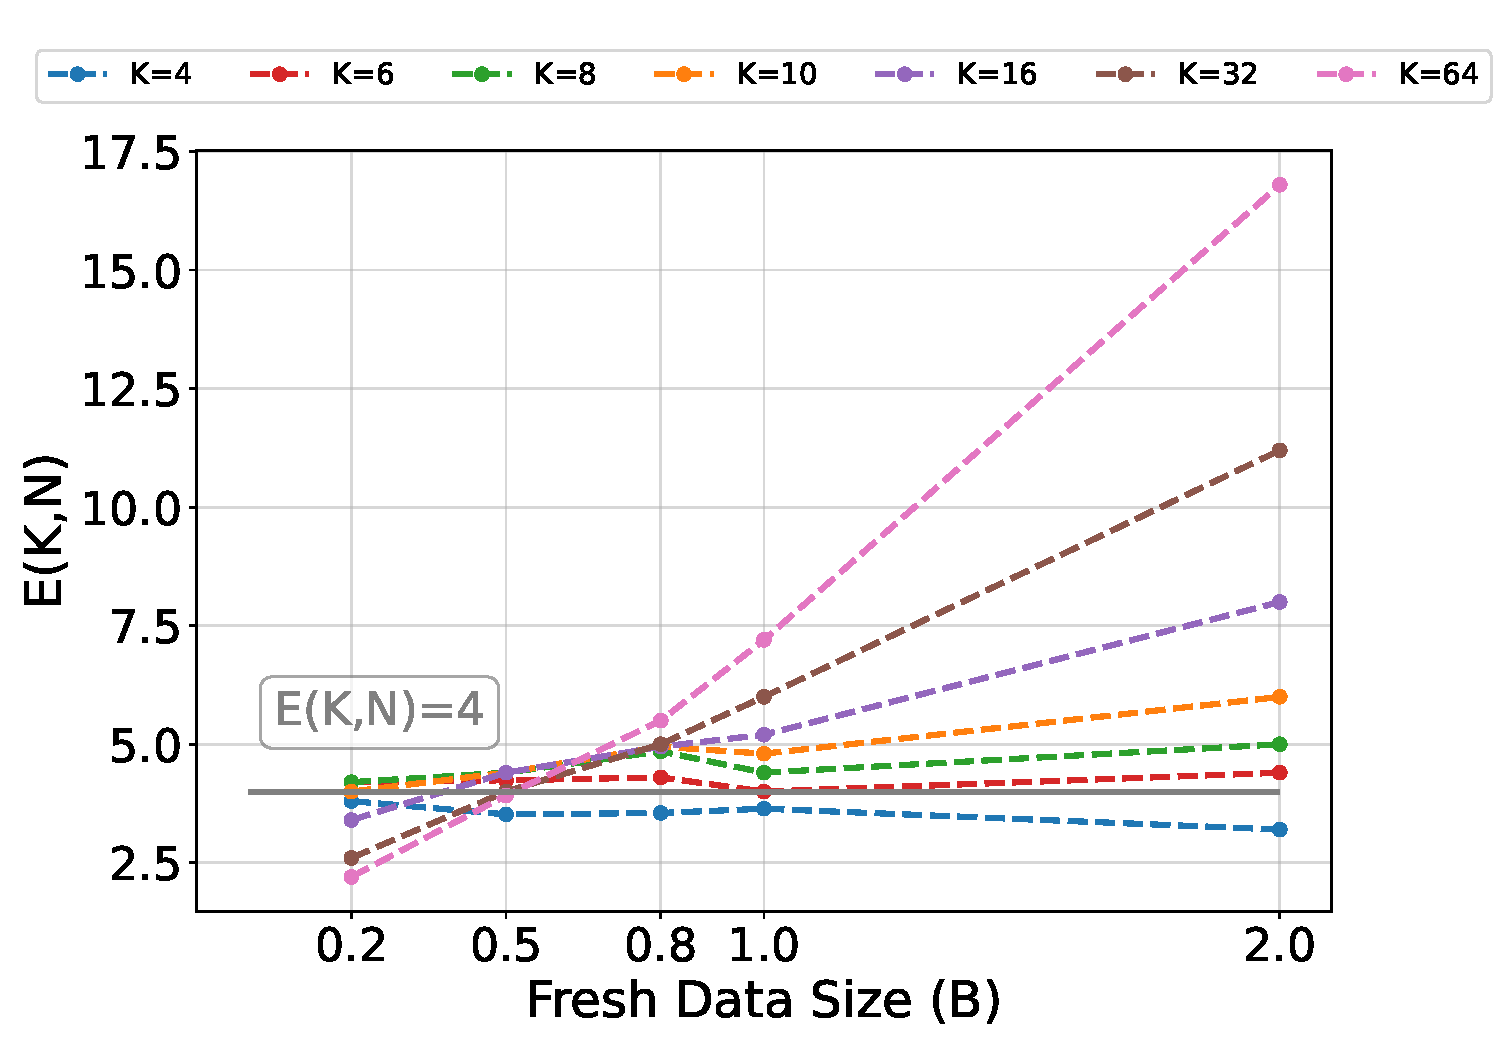
\includegraphics[width=\linewidth]{figs/E_k_over_fresh_data_size.pdf}
        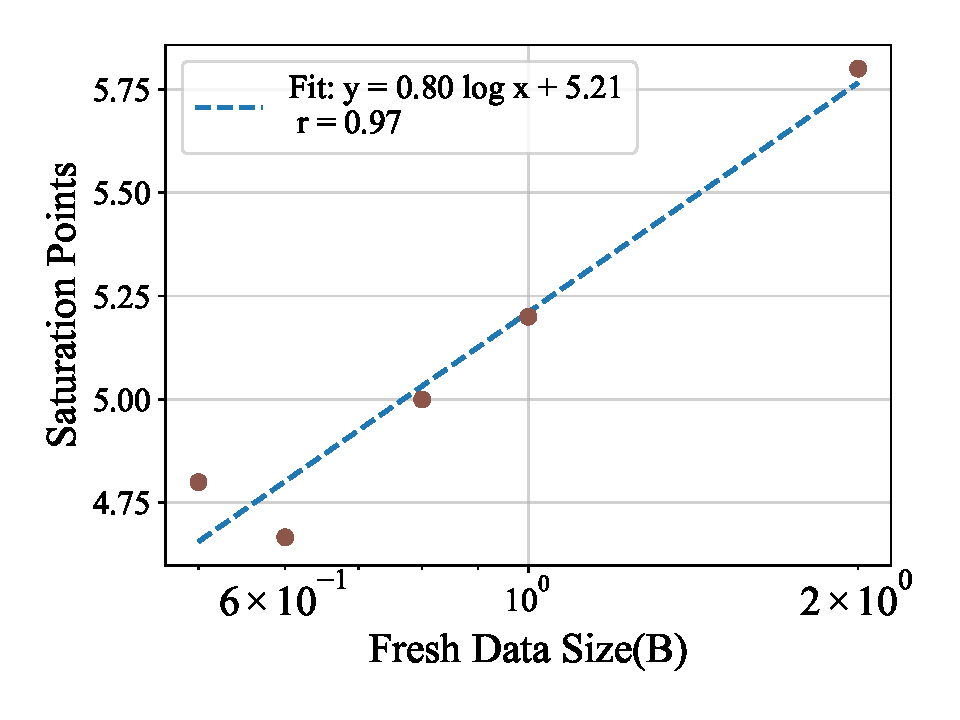
\includegraphics[width=\linewidth,trim=0 0.22in 0 0,clip]{figs/E_KN_vs_N_ws3_ratio0.75_alpha0.9_exp.pdf}
        \caption{The saturation points grows linearly with $\log N$.}
        %\caption{The saturation points $K(\lambda,N)$ as a function of the dataset size N.}
        \label{fig:ek-n-saturation point}
    \end{subfigure}
    \caption{\small Our LLM experiments show that larger datasets can be repeated more.
    \textbf{(a)} The effective reuse rate $E(K, N) \approx K$ when $K$ is small, but eventually saturates at certain number of epochs. \textbf{(b)} The saturation point shifts to larger $K$ as the dataset size increases. \textbf{(c)} Empirically, the saturation points scales linearly with $\log N$.} \label{fig:main-llm}
    %The effective reuse rate $E(K,N)$ over $K$ and training curves in our language model experiments. \Cref{fig:ek-k} shows that $E(K,N)\approx K$ when $K$ is small, to be specific, $K\leq4$. \Cref{fig:loss-step} plots the points where $E(K,N)=0.8K$ under different configurations, and we define the corresponding $E(K,N)$ as the saturation points. In \Cref{fig:ek-n-saturation point}, we observe that the saturation points increases as $N$ increases, indicating that larger datasets can be repeated more.}
    % \kaifeng{you didn't mention figure c}}
    % \caption{}
    % \caption{\textbf{Left:} Training loss progression over training steps. \textbf{Right:} The saturated effective reuse rate $E(K,N)$ in relation to the size of the fresh dataset $N$.}
    \vspace{-0.1in}
\end{figure}

%Then we define the minimum $N'$ such that $\mathcal{L}(1, N') \leq \mathcal{L}(K, N)$, and interpret the ratio $E(K, N) = N'/N$ as the effective reuse rate of the data (see the detailed version in Definition~\ref{def:E_K}).

In a recent study of scaling laws for multi-epoch training, \citet{muennighoff2023scaling} encountered this question and proposed an empirical approximation: $N'(K, N) = \left(1 + R^* (1 - e^{-(K-1)/R^*})\right) \cdot N$,
%Recently, \citet{muennighoff2023scaling} provided an empirical approximation to this key quantity.
%Previous work has provided empirical approximations to this key quantity.
%In particular, \citet{muennighoff2023scaling} proposed to approximate the effective dataset size as
where $R^*$ is a fitted constant ($R^* \approx 15.39$ in their experiments).
This formula suggests that the benefit of repetition grows with $K$ but saturates exponentially at $(1 + R^*) \cdot N$ as $K$ increases. While supported by some empirical evidence in their study, this approximation still leads to a noticeable gap between scaling law predictions and empirical results (see Figure 3 in their paper). Moreover, the formula implies that the ratio $E(K,N) = N'(K, N)/N$ is independent of $N$, so the benefit of repeating the dataset $K$ times is equivalent to increasing its size by a factor that depends only on $K$, regardless of how large $N$ is. It remains unclear to what extent this independence holds in general.


%though it still leaves a noticeable gap between predicted scaling behavior and observed performance, and critically assumes that the ratio $N'(N, K)/N$ is independent of $N$. 

\paragraph{Our Contributions.}
In this paper, we approach the above question on the effective reuse rate of data in the setting of linear regression, a setting that is simple enough to reveal the key mechanisms of data reuse, while still tractable for precise analysis under stochastic gradient descent (SGD).
We provide a theoretical characterization of $E(K, N)$ in various regimes, and point out a neglected factor in the empirical study of \citet{muennighoff2023scaling}: the effective reuse rate depends not only on the number of epochs $K$, but also on the dataset size $N$.
In fact, we show both theoretically and empirically that \textbf{larger datasets can be repeated more}.
%in the setting of linear regression, which is simple enough to reveal the key mechanisms of data reuse, while still tractable for precise analysis under stochastic gradient descent (SGD).
%present a theoretical analysis on the scaling behavior of multi-epoch training in linear regression, and
%provide a theoretical characterization of how $E(K, N)$ depends jointly on $K$ and $N$, complementing prior empirical observations with a principled perspective.
%increase the effective dataset size under one-pass training?}
% \begin{center}
%     \textit{To what extent does training for $K$ epochs on $N$ samples increase the effective dataset size under one-pass training?}
% \end{center}
% \haodong{keep it or not, put it in the line}
% \begin{align}
%     N' = \left(1 + R^* (1 - e^{-(K-1)/R^*})\right) \cdot N,\label{equ:data-constrained-EK}
% \end{align}
%\haodong{rephrase the following paragraph Binghui}
% In contrast, our analysis provides a theoretical characterization of how $E(K, N)$ depends jointly on $K$ and $N$, complementing prior empirical observations with a principled perspective.
% To our knowledge, this work constitutes the first systematic investigation of data scaling laws in the multi-epoch training regime. 
% In this work, under a linear regression setup, we theoretically analyze the data scaling behavior in the multi-epoch training regime. 
%We approach this question in the setting of linear regression, which is simple enough to reveal the key mechanisms of data reuse, while still tractable for precise analysis under stochastic gradient descent (SGD). This makes it a natural testbed for developing a theoretical understanding of multi-epoch scaling. 
%Specifically, we focus on two cases: the strongly convex setting and the high-dimensional setting with a Zipf-law data distribution. 
Our main contributions are as follows:
\begin{enumerate}
\item In~\Cref{sec:strongly_convex}, we analyze multi-epoch SGD for linear regression under strong convexity.
We show that when $K$ is small, $E(K, N) \approx K$, so every new epoch leads to a linear gain. As $K$ increases, $E(K, N)$ saturates at a problem-dependent value of order $\Theta(\log N)$, suggesting that larger datasets can be repeated for more epochs before the marginal benefit vanishes.

\item In~\Cref{sec:one_hot}, we go beyond the strongly convex case and study a class of Zipf-law distributed data, and show that $E(K, N)$ exhibits a similar scaling behavior to the strongly convex case, except that the saturation point scales as a power of $N$ instead of $\log N$.

\item Technically, we derive the optimal learning rate (Lemma~\ref{thm:convex-opt-lr}) for multi-epoch SGD in linear regression and its corresponding approximation formula for the expected excess risk up to an $o(1)$ multiplicative error (Lemma~\ref{thm:convex-L-estimate}). These results may be of independent interest.

\item In~\Cref{sec:experiments}, we conduct LLM pretraining experiments with up to $200$B repeated tokens.
Consistent with our theoretical findings, the empirical results show that $E(K, N) \approx K$ for small $K$, but eventually saturates at an epoch number that scales linearly with $\log N$. 
See also~\Cref{fig:main-llm} for details.
\end{enumerate}

%Our empirical results show that $E(K, N) \approx K$ for small $K$ 
%Similar to our findings in the strongly convex case of linear regression, the saturation point scales linearly with $\log N$.
%We establish  characterization of multi-epoch data scaling in linear regression. We show that $E(K, N) \approx K$ for small $K$, reflecting nearly linear gains from repetition, while for large $K$ the effective reuse rate saturates at an $N$-dependent level: proportional to $\log N$ in the strongly convex case and to $N^\alpha$ (for some $\alpha \in (0,1)$) in the Zipf-law case. This reveals that larger datasets can be repeated more effectively, with the saturation point determined by the problem setup.
%\item We technically provide the first theoretical characterization of the optimal learning rate for multi-epoch SGD in linear regression. This is enabled by a new approximation formula for the expected excess risk up to an $o(1)$ multiplicative error (Lemma~\ref{thm:convex-L-estimate}), which also allows for a tractable analysis of optimal learning rate schedules (Lemma~\ref{thm:convex-opt-lr}). These technical results may be of independent interest.
%This provides direct evidence for our main conclusion: larger datasets can be repeated more.
%We empirically validate our theoretical predictions through LLM pre-training experiments. The results confirm that $E(K, N) \approx K$ for small $K$, and that for fixed $K$, the effective reuse rate increases monotonically with $N$. This provides direct evidence for our central conclusion: larger datasets can indeed be repeated more effectively.
% Our main contributions can be summarized as follows:
% \begin{enumerate}
%     \item 
%     In Section~\ref{sec:strongly_convex}, our analysis in the strongly convex case of linear regression shows that, if the learning rate is optimally tuned, $E(K, N)$ grows proportionally to $\log N$ and saturates at $K$ when $\log N \gg K$ (Theorem~\ref{thm:convex-E_K}).
%     \item Technically, we provide an approximation formula for the expected excess risk up to $o(1)$ multiplicative error~(Lemma~\ref{thm:convex-L-estimate}), which enables a tractable analysis of the optimal learning rate (Lemma~\ref{thm:convex-opt-lr}). These results may be of independent interest.
%     \item 
%     In ~\Cref{sec:one_hot}, we consider a solvable case with a power-law spectrum structure. Under this setting, we prove that $E(K, N)$ exhibits a similar scaling behavior to the strongly convex case, but it has different saturation points for different spectra (\Cref{thm:one-hot-E_K-v2} and \Cref{thm:one-hot-E_K-log-spectrum}).
%     \item 
%     In Section~\ref{sec:experiments}, we validate our theoretical implications in the context of language model pretraining. Our findings indicate that the effective reuse rate approximates the epoch number for small numbers of repetitions. Furthermore, for a fixed number of epochs, the effective reuse rate increases monotonically with the fresh data size (\Cref{fig:ek-k,fig:ek-data,fig:loss-step}). This supports the conclusion that larger datasets can be repeated more effectively.
% \end{enumerate}

% When developing scaling laws for multi-epoch training,~\citet{muennighoff2023scaling} encountered this question and proposed the following approximation for the effective data size $N'$: 
% % $N' = \left(1 + R^* (1 - e^{-(K-1)/R^*})\right) \cdot N$,
% \begin{align}
%     N' = \left(1 + R^* (1 - e^{-(K-1)/R^*})\right) \cdot N,\label{equ:data-constrained-EK}
% \end{align}
% where $R^*$ is a fitted constant ($R^* \approx 15.39$ in their experiments). This formula suggests that the benefit of repetition grows with $K$ but saturates exponentially at $(1 + R^*) \cdot N$ as $K$ increases. While supported by some empirical evidence in their study, this approximation still leads to a noticeable gap between scaling law predictions and empirical results (see Figure 3 in their paper).
% Moreover, the formula implies that the ratio $N'/N$ is independent of $N$, so the benefit of repeating the dataset $K$ times is equivalent to increasing the dataset size by a factor that depends only on $K$, regardless of how large $N$ is. It remains unclear to what extent this independence holds in general.

%Notably, the formula implies that the ratio $N' / N$ is independent of $N$. This means that no matter how large the dataset size $N$ is, the benefit of repeating the dataset $K$ times is equivalent to increasing the dataset size by a factor that depends only on $K$.
%and it is also unclear to what extent this formula holds more broadly.

%Notably, the formula implies that the fraction $N' / N$ is always a constant in $N$, and thus no matter how large the dataset size $N$ is, repeating the dataset $K$ times always benefits the performance like multiplying the dataset size by a factor only depending on $K$.



%This formula assumes that when repeating the dataset, the effective dataset size grows with the number of epochs $K$, but the growth exponentially saturates to $(1 + R^*) \cdot N$ as $K$ becomes much larger than $R^*$. However, although some empirical evidence is presented in~\citet{muennighoff2023scaling}, it is not clear whether this form of $N'$ is universally applicable to all practical settings. In particular, in this formula, 


% \paragraph{Our Contributions.}
% In this paper, we present a theoretical analysis on the scaling behavior of multi-epoch training and examine how $N'/N$ really behaves in linear regression problems.
% Formally, we define the {\it effective reuse rate} $E(K, N)$ of the data as $N'/N$, the ratio of the effective dataset size $N'$ to the original dataset size $N$ for $K$-epoch training (see the formal definition in Definition~\ref{def:E_K}). Our main contribution can be summarized as follows:
% \begin{enumerate}
%     \item 
%     In Section~\ref{sec:strongly_convex}, our analysis in the strongly convex case of linear regression shows that, if the learning rate is optimally tuned, $E(K, N)$ grows proportionally to $\log N$ and saturates at $K$ when $\log N \gg K$ (Theorem~\ref{thm:convex-E_K}).
%     %\item Technically, we provide an approximation formula for the expected excess risk up to $o(1)$ multiplicative error~(Lemma~\ref{thm:convex-L-estimate}), which enables a tractable analysis of the optimal learning rate (Lemma~\ref{thm:convex-opt-lr}). These results may be of independent interest.  % \kairong{What is ``population excess risk''? Is it a well-known term?} \kairong{Fine, find it in Preliminary.}
%     %Then, based on the approximately optimal learning rate for one-pass SGD and the designed learning rate for multi-epoch SGD, we show that $E(K, N)$ grows proportionally to $\log N$ and saturates at $K$ when $\log N \gg K$ (Theorem~\ref{thm:convex-E_K}).
%     \item 
%     In ~\Cref{sec:one_hot}, we consider a solvable case with a power-law spectrum structure. Under this setting, we prove that $E(K, N)$ exhibits a similar scaling behavior to the strongly convex case, but it has different saturation points for different spectra (\Cref{thm:one-hot-E_K-v2}).%, \Cref{thm:one-hot-E_K-log-spectrum}, and \Cref{thm:one-hot-E_K-b=0}).
%     \item 
%     In Section~\ref{sec:experiments}, we validate our theoretical implications in the context of language model pretraining. Our findings indicate that the effective reuse rate approximates the epoch number for small numbers of repetitions. Furthermore, for a fixed number of epochs, the effective reuse rate increases monotonically with the fresh data size (\Cref{fig:ek-k,fig:ek-data,fig:loss-step}). This supports the conclusion that larger datasets can be repeated more effectively.
% \end{enumerate}

%Noting that $N'$ may take the form of $N$ multiplied by a factor, in this paper, we stu
%provide an extensive empirical study of the scaling behavior of multi-epoch training, and propose that training a model on a dataset of size $N$ for $K$ epochs leads to a loss similar to that of training on a dataset of size $N'$ in the one-pass regime, where the {\it effective dataset size} $N'$ is given by
% \begin{align}
%     N' = \left(1 + R^* (1 - e^{-(K-1)/R^*})\right) \cdot N,
% \end{align}

%where $R^*$ is a constant to be fit from empirical experiments ($R^* \approx 15.39$ in their experiments). This formula assumes that when repeating the dataset, the effective dataset size grows with the number of epochs $K$, but the growth exponentially saturates to $(1 + R^*) \cdot N$ as $K$ becomes much larger than $R^*$. However, although some empirical evidence is presented in~\citet{muennighoff2023scaling}, it is not clear whether this form of $N'$ is universally applicable to all practical settings, and whether $R^*$ is indeed a constant independent of other factors.


%the form of $R^*$ and its dependence on the dataset size, model size, and number of passes $K$ is not well understood.
%, assumed to be independent of the dataset size, model size, and number of passes $K$ 

%That is, the 
%the effective dataset size under repetition can be expressed as $C_K \cdot N$, where $C_K$ is a constant potentially dependent on the number of passes $K$, but its form and behavior remain unclear. 
%study the effect of ME training on scaling laws and observe that for a small number of epochs, repeated data can approximate the benefits of fresh data. However, their findings also reveal a clear degradation: as the number of epochs increases—e.g., beyond four passes over 900 billion tokens—performance gains diminish, and the marginal utility of additional compute approaches zero.

%\citet{charton2024emergent} and 

%These results highlight the empirical limitations of ME training at scale. Yet, despite its practical relevance, our theoretical understanding of how data repetition influences scaling laws remains limited. In particular, there is a lack of rigorous derivations capturing this behavior. For example, \citet{muennighoff2023scaling} suggest that the effective dataset size under repetition can be expressed as $C_K \cdot N$, where $C_K$ is a constant potentially dependent on the number of passes $K$, but its form and behavior remain unclear. Moreover, existing scaling formulas derived in the OP regime fail to extrapolate accurately as $K$ becomes large.

%In this paper, we study the scaling behavior of multi-epoch training from a theoretical perspective. 
%Concretely, 


%To study how $N'$ behaves in the data-constrained regime, we introduce the notion of effective reuse rate, which we define as the factor by which the dataset must grow under one-pass training to match the test loss of multi-epoch training.
%denoted $E(K, N)$


%, as a principled measure of how repeated exposure to a finite dataset contributes to training. This term generalizes the idea of effective dataset size and serves as a core quantity for analyzing scaling behavior in the data-constrained regime.


%Motivated by these limitations, we revisit the problem of multi-epoch training from an information-theoretic perspective. We introduce the notion of effective reuse rate, denoted $E(K, N)$ (see the formal definition in Definition~\ref{def:E_K}), as a principled measure of how repeated exposure to a finite dataset contributes to training. This term generalizes the idea of effective dataset size and serves as a core quantity for analyzing scaling behavior in the data-constrained regime.

%\begin{center}
%\textit{Can we provably characterize the scaling behavior of $E(K, N)$ in the data-constrained regime?}
%\end{center}


% \kaifeng{reorganize into bullet points}
% In this paper, we study the theory of the scaling behavior differences between one-pass (OP) and multi-epoch (ME) training in two classical linear regression setups. We provide a theoretical framework for analyzing \( E(K, N) \) under solvable models, offering insight into how compute and data interact when data reuse is unavoidable. The first model we consider is a finite-dimensional, strongly convex linear regression problem, for which we apply both OP stochastic gradient descent (SGD) and ME SGD algorithms. We perform a fine-grained analysis of the population excess risk for both optimization algorithms and analyze the scaling behavior of these two algorithms under a selected learning rate, achieving an approximately optimal convergence rate for OP SGD. The second problem we investigate is an infinite-dimensional linear regression problem, with a power spectrum assumption on the covariance matrix, which is commonly used in scaling law theory~\citep{lin2024scaling,luo2025multi}. We derive matching upper and lower bounds for the loss obtained by both ME and OP SGD optimization algorithms, thus providing an expression for the scaling law.


%\paragraph{Motivation.} The motivation of our theory is to derive the effective number of epochs. In other words, if we run an ME SGD for $K$ epochs, how many effective epochs would be required for the corresponding OP to achieve the saME population excess risk as ME? Specifically, considering an ME SGD optimization algorithm with dataset size $N$, and number of epochs $K$, and the ME SGD after $T=KN$ steps achieves a population excess risk $L_T$, correspondingly, we have another OP SGD, with unique data in every step, runing $T'$ steps, with population excess risk $L'_{T'}$. Now we select the minimal $T'$ such that $L'_{T'} \le L_T$, and we define the term $E_K=T'/N$ as the effective number of epochs, which characterizes the difference between ME and OP in their scaling behaviors.

%\paragraph{Challenge.}\haodong{it is typically hard to directly analyze the loss formula and get the clean expression of $E_K$. Also, the iMEact of random shuffling is extreMEly tedious to capture.}

% \paragraph{Our Contribution.}
% \begin{itemize}
%     \item Considering random shuffling, give a mathematical fraMEwork for multi-epoch SGD in standard finite diMEnsion strongly convex linear regression, provide results like: loss approximation, with tools in matrix concentration, asyMEtotically optimal learning rate, and effective number of epochs.
%     \item In power spectrum assuMEtion (non-strongly convex case) with top $d$ sketching matrix $S$, we get: loss approximation (scaling law), and 
% we give an analysis of the effective number of epochs with soME learning rate.
% \end{itemize}

% Our main contributions are sumMErized as follows.
% \begin{itemize}
%     \item 
%     formalize $E_K$ xxx
%     \item 
%     strongly convex linear regression xxx
%     \item 
%     one-hot power law xxx
%     \item 
%     in real-world experiMEnts xxx
% \end{itemize}